
%%%%%%%%%%%%%%%%%%%%%%%%%%%%%%%%%%%%%%%%%%%%%%%%%%%%%%%%%%%%%%%%%%%%%%%%%
%
% File: JEODcoord.tex
%
% Purpose: Top level document for Model.  Should not need to be edited.
%
%%%%%%%%%%%%%%%%%%%%%%%%%%%%%%%%%%%%%%%%%%%%%%%%%%%%%%%%%%%%%%%%%%%%%%%%%

\documentclass[twoside,11pt,titlepage]{report}

%
% Bring in the common page setup
%
\usepackage{dynenv}

%
% Bring in the model-specific commands
%
\usepackage{COORDFRAME}

%
% Bring in the graphics environment
%
\usepackage{graphicx}
\usepackage{appendix}
\usepackage{wasysym}
%
% Bring in the hyper ref environment
%
\usepackage[colorlinks,plainpages=false]{hyperref}
%  keywords for pdfkeywords are separated by commas
\hypersetup{
   pdftitle={\COORDFRAMEDesc},
   pdfauthor={\ModelAuthor},
   pdfkeywords={\ModelKeywords},
   pdfsubject={\COORDFRAMEDesc}}

% for document revisions only: 
\newcommand\documentHistory{
{\bf Author} & {\bf Date} & {\bf Description} \\ \hline \hline
A. A. Jackson & March 2012 &  Initial Version \\ \hline
}


\begin{document}

%%%%%%%%%%%%%%%%%%%%%%%%%%%%%%%%%%%
% Front matter
%%%%%%%%%%%%%%%%%%%%%%%%%%%%%%%%%%%
\pagenumbering{roman}

\docid{docs}
\docrev{1.0}
\date{\RELEASEMONTH\ \RELEASEYEAR}
\modelname{\COORDFRAMEDesc}
\doctype{}
\author{\ModelAuthor}
\managers{
  Robert O. Shelton \\ Project Manager \\
  Michael T. Red \\ Simulation and Graphics Branch Chief \\
  R. Matt Ondler \\ Software, Robotics, and Simulation Division Chief}
\pdfbookmark{Title Page}{titlepage}
\makeDynenvTitlepage

\pdfbookmark{Abstract}{abstract}
%%%%%%%%%%%%%%%%%%%%%%%%%%%%%%%%%%%%%%%%%%%%%%%%%%%%%%%%%%%%%%%%%%%%%%%%
%Planet Fixed Utility
% Purpose:
%
% 
%
%%%%%%%%%%%%%%%%%%%%%%%%%%%%%%%%%%%%%%%%%%%%%%%%%%%%%%%%%%%%%%%%%%%%%%%%%

\begin{abstract}
This document describes the \JEOD  ~coordinate systems:
Described here are the coordinate frames used for solar system bodies and for those frames associated with a spacecraft or multibody spacecraft. The coordinate systems are defined and illustrated. The agencies which specify these systems are identified. Examples of the use of these systems in \JEOD are presented.

\end{abstract}

\setcounter{chapter}{0}
\pdfbookmark{Contents}{contents}
\tableofcontents
\vfill
%----------------------------------
\chapter{Introduction}\hyperdef{part}{intro}{}\label{ch:intro}
%----------------------------------
\pagenumbering{arabic}

%sections{Document Description}


\section{Document History}
%%% Status of this and only this document.  Any date should be relevant to when 
%%% this document was last updated and mention the reason (release, bug fix, etc.)
%%% Mention previous history aka JEOD 1.4-5 heritage in this sections.
%%% Mention that JEOD.pdf is the parent document.

\begin{tabular}{||l|l|l|} \hline
\documentHistory
\end{tabular}

\section{Document Organization}
This document is formatted in accordance with the 
NASA Software Engineering sections Standard~\cite{NASA:SWE} 

\section{Coordinate Frames Introduction}
 A reference frame is an ordered set of three
mutually orthogonal (possibly time dependent) unit length
direction vectors, coupled with a location
called the frame's center or origin.
 
Astrodynamics standards distinguish between a reference system and a reference frame \cite{IAU2006}.
(1) A reference system is the complete specification of how a celestial coordinate
or vehicle system is to be formed. It defines the origin and fundamental planes (or axes) of the coordinate system. It also specifies all of the constants, models, and algorithms used to transform between observable quantities and reference data that conform to the system.
(2) A celestial reference frame consists of a set of identifiable fiducial points on the sky along with their coordinates, which serves as the practical realization of a reference system.

In addition vehicle associated reference frames are defined when necessary.

\paragraph{Authority Standards} 
\begin{itemize}
\item {Planetary Data System (PDS) - Jet Propulsion Laboratory (JPL) and the 
JPL Navigation and Ancillary Information Facility }
\item { International Astronomical Union (IAU)
The IAU Working Group on Cartographic coordinates.
     Coordinates and Rotational Elements
(Coordinated with JPL's Development Ephemeris) }
\end{itemize}

\paragraph{Notes}
\begin{itemize}
\item {In the following IERS stands for International Earth Rotation Service.}
\item{ In anticipation of the expansion of JEOD celestial coordinate systems to bodies other than the Earth, Moon and Mars sections 2 and 3 below 
are presented to be in conformance with
the IAU\cite{IAU2006} and IERS \cite{IERS2003}.

Because of their generality these systems are presented in the order that follows. The Generalized system is presented first and a more detalied realization is presented following.}
\end{itemize}


%\end{description}

%----------------------------------
%\chapter{JEOD Coordinate Systems}\hyperdef{part}{reqt}{}\label{ch:coord}\JEODid}
%----------------------------------
\chapter{JEOD Coordinate Systems}

\nopagebreak
\section{International Celestial Reference System-ICRF and the Barycentric Celestial Reference System - BCRF} \label{sec:bcrf} 

The International Celestial Reference System (ICRS) is the current standard celestial reference system adopted by the International Astronomical Union (IAU). Its origin is at the barycenter of the solar system, with axes that are intended to be "fixed" with respect to space. ICRS co-ordinates are approximately the same as equatorial coordinates, the mean pole at J2000 \cite{IERS2003}. The International Celestial Reference Frame (ICRF) is defined by a catalog of adopted positions of 608 extragalactic radio sources, 212 of them defining the ICRS axes. The BCRF is a system of barycentric space-time coordinates for the solar system within the framework of General Relativity with metric tensor specified by the IAU 2003 Resolution \cite{IERS2003}. Formally, the metric tensor of the BCRS does not fix the coordinates completely, leaving the final orientation of the spatial axes undefined. However, for all practical applications, unless otherwise stated, the BCRS is assumed to be oriented according to the International Coordinate System, ICRS axes \cite{IERS2003}. The JEOD barycenter coordinates are the same as the JPL system that is: the origin of the rectangular coordinates is at the solar system barycenter (center of mass) for the Sun and all planets, except the Earth, figure \ref{fig:1}. Note for all the astronomical systems and associated epoch must be given, see the \hypermodelref{TIME}. 

\textbf{Coordinate Frame Center: }Solar System Barycenter. 

\textbf{Coordinate Frame: } Non-Rotating Inertial

\begin{itemize}
\item X-axis: Defined as the cross product of the Z-axis (as defined below) and the Earth mean orbit pole of J2000 (i.e. the ecliptic pole of J2000). The X-axis of this coordinate frame is the Earth vernal equinox of J2000.
\item Y-axis: Completes a standard, right-handed coordinate frame.
\item Z-axis: Defined as the pole vector of the Earth Mean Equator of J2000 (where J2000 = Julian date 2451545.0).
\end{itemize}

\newpage
\begin{figure}[!ht]
\centering
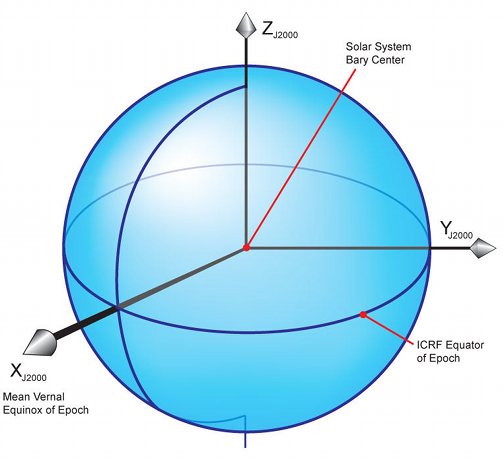
\includegraphics [width=7in]{figs/fig1.png}
\caption{The ICRF and BCRF System}
\label{fig:1}
\end{figure}

\subsection{ICRF and BCRF Example}
To know the position of the Sun and Moon, for example, one must set up a sim\_object in the S\_define file , for instance in SIM 4 in the \hyperTutorial. Let the JPL ephemerides be DE421. The entry is then:
\begin{verbatim}
environment/ephemerides/de4xx_ephem:  De4xxEphemeris de421
      (environment/ephemerides/de4xx_ephem/data/de421.d);
\end{verbatim}
In this example the multibody gravitational forces from the Sun and Moon need to be invoked. In the Modified Data directory for Tutorial Sim 4 the following lines should be set:

\begin{verbatim}
/* Set up the gravity controls for the Sun. */
VEH_OBJ.sun_grav_ctrl.planet_name   = "Sun";
VEH_OBJ.sun_grav_ctrl.active        = True;
VEH_OBJ.sun_grav_ctrl.spherical     = True;

/* Set up the gravity controls for the Moon. */
VEH_OBJ.moon_grav_ctrl.planet_name  = "Moon";
VEH_OBJ.moon_grav_ctrl.active       = True;
VEH_OBJ.moon_grav_ctrl.spherical    = True;
\end{verbatim}





\section{General Solar System Inertial and Fixed Systems} \label{sec:gen} 
Established here is the generic coordinate system of solar system bodies as set by the International Astronomical Union \cite{IAU2006} and adopted by the PDS.  The IAU system applies to all bodies in the solar system. The IAU defined transformation from inertial to body fixed is given by a simple formulation for all solar system bodies. The general ICRS is a coordinate system with its origin at the solar system body center and axis directions that are defined as parallel to those of the ICRS system. See section \ref{sec:bcrf} for definition of the ICRS and section \ref{sec:gendet} for a more formal relation between inertial and rotating system.

In JEOD more refined and sophisticated body orientation parameters are needed for non-spherical gravitational fields. In particular the transformation from inertial to body fixed exist for the Earth, Moon and Mars, the reader is referred the relevant body orientation system for these bodies, see \hypermodelref{TIME}\  for the Earth and Mars and \hypermodelref{EPHEMERIDES} for the Moon.  For all other bodies such planets, asteroids, satellites and dwarf planets, only the IAU orientation parameters are currently included in JEOD. 

Figure \ref{fig:2} presented here is the IAU cannonical standard or IAU generic fixed coordinate frame. The pole is specified as the two intersection points of the body's equator and the ICRF equator define it as the node Q. The prime meridian has been chosen so that it crosses the body's equator at point B.\\
\begin{itemize}
\item $\alpha_0$ = right ascension of pole.\\
\item $\delta_0$ = declination of the pole.\\
\item $\aries$  is the direction of Ares at epoch J2000.\\
\item W = location of the prime meridian Q with respect to B.\\
\end{itemize}
\textbf{Coordinate Frame: } IAU generic fixed.

\begin{itemize}
\item X-axis: Defined as the cross product of the Z-axis (as defined below) and the Earth mean orbit pole of J2000 (i.e. the ecliptic pole of J2000). The X-axis of this coordinate frame is the
Earth vernal equinox of J2000.
\item Y-axis: Completes a standard, right-handed coordinate frame.
\item Z-axis: Defined as the pole vector of the Earth Mean Equator of J2000
(where J2000 = Julian date 2451545.0).
\end{itemize}


\begin{figure}[htp]
\centering
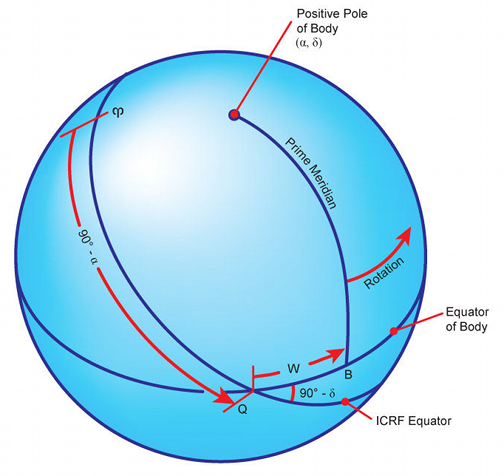
\includegraphics [width=7in]{figs/fig2.png}
\caption{IAU Pole and Meridian Definitions}
\label{fig:2}
\end{figure}

\subsection{Example General IAU Body System}
See section \ref{sec:gendet} for elaboration.





\section{The IAU Solar System Body Centered Orientation } \label{sec:gendet} 
This section is an elaboration of the basic IAU system defined in Section 2.
Planetary coordinate systems are defined relative to their mean axis of rotation and various definitions of longitude depending on the body. The longitude systems of most of those bodies with observable rigid surfaces have been defined by references to a surface feature such as a crater. Approximate expressions for these rotational elements with respect to the ICRF have been derived. 
The north pole is that pole of rotation that lies on the north side of the invariable plane of the solar system. The direction of the north pole is specified by the value of its right ascension $\alpha_0$ and declination $\delta_0$. With the pole so specified, the two intersection points of the body's equator and the ICRF equator are $\alpha_0$ +90, define it as the node Q. Suppose the prime meridian has been chosen so that it crosses the body's equator at point B. Then specify the location of the prime meridian by providing a value for W, the angle measured easterly along the body's equator between the node the first sign of Aries $\aries$ and the intersection of the body equator and the ICRF equator (see Fig. 3). The right ascension of the point is 90. + $\alpha_0$ and the inclination of the planet's equator to the celestial equator is 90-$\alpha_0$. As long as the planet, and hence its prime meridian, rotates uniformly,W varies nearly linearly with time. In addition, $\alpha_0$, $\delta_0$, and W may vary with time due to a precession of the axis of rotation of the body (or satellite). If W increases with time, the body has a direct (or prograde) rotation, and, if W decreases with time, the rotation is said to be retrograde.
Bodies without solid surfaces are very irregular solid surfaces, all have a prime meridian but have to be chosen in different ways , see the IAU publication \cite{IAU2006}.

\textbf{Coordinate Frame: } Rotating

\begin{itemize}
\item X - axis: Out the prime meridian.
\item Y - axis: Completes the right-handed system.
\item Z - axis: Defined as the pole vector of the body of interest, with epoch J2000 (where J2000 = Julian date 2451545.0 TDB (Barycentric Dynamical Time)). 
\end{itemize}
The north pole is that pole of rotation lies on the north side of the invariable plane of the solar system.

\begin{figure}[htp]
\centering
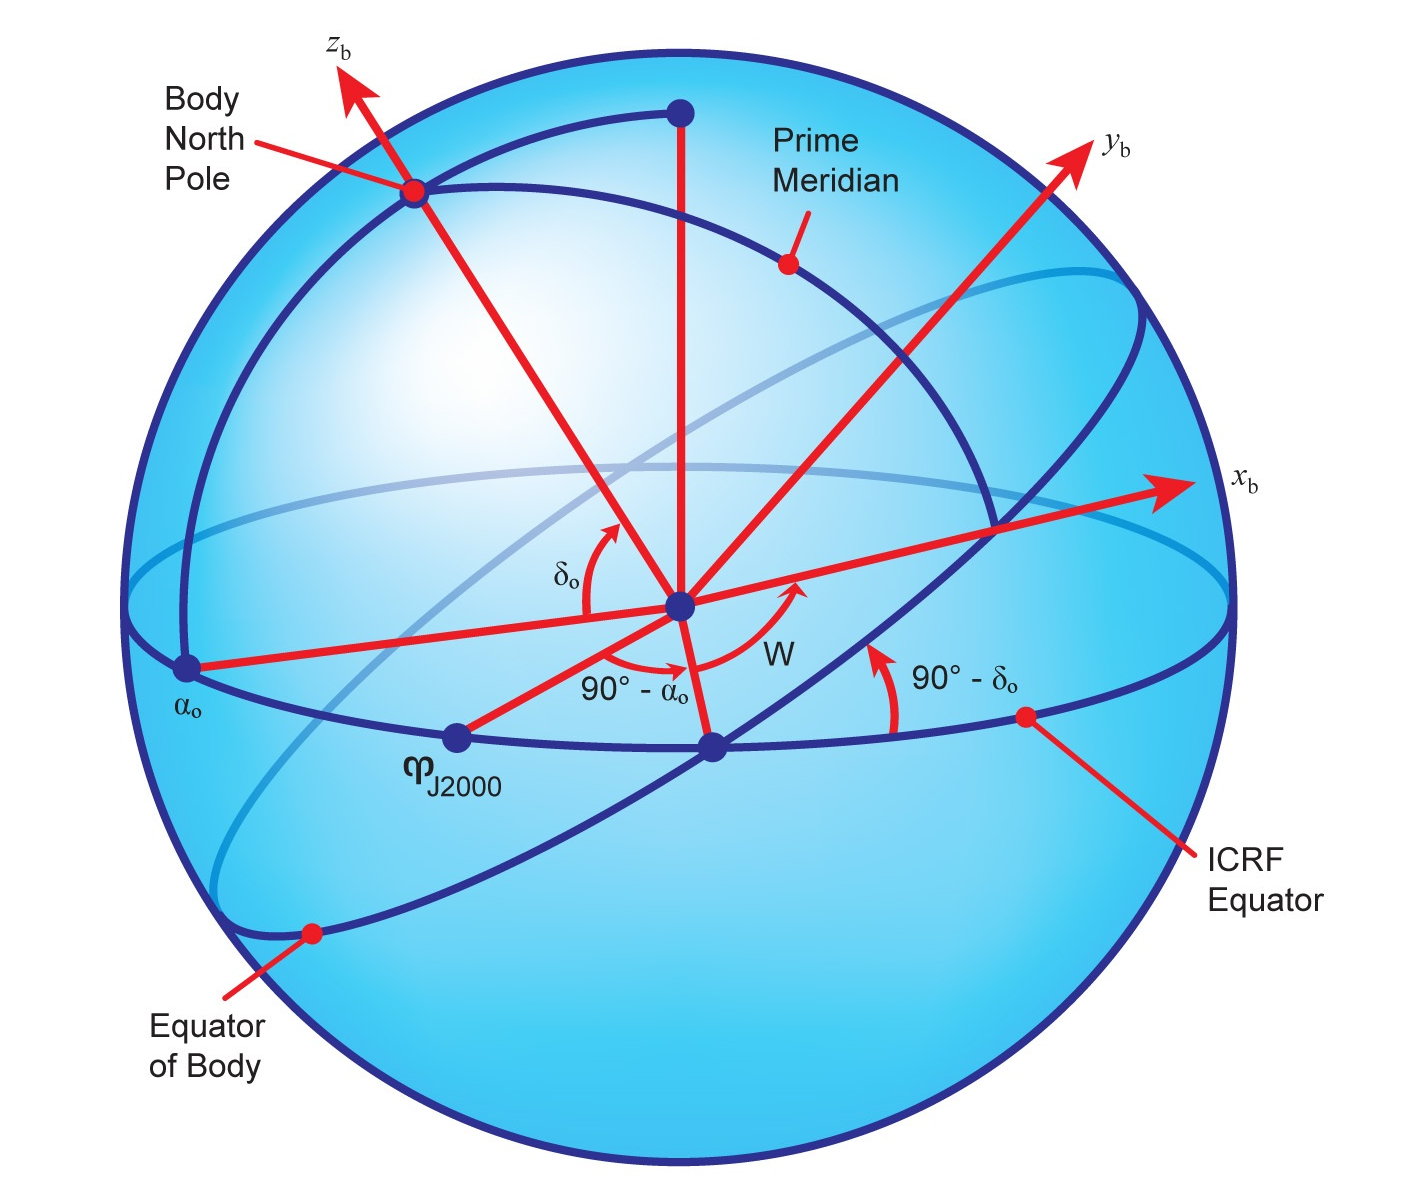
\includegraphics [width=7in]{figs/fig3.png}
\caption{Realization of the IAU Fixed Body Reference System}
\label{fig:3}
\end{figure}

\newpage
\subsection{Example IAU Body Centered}

The following rotation is used by the Planetary Data System (PDS) to transform 
from ICRF inertial to body fixed. The IAU specifies a simple formulation for $\alpha$,
$\beta$, , W and the rates of change of these parametes ,these can be either constands or a
and expansion in a periodic series \cite{IAU2006}.
The PDS rotation matric R is:

\begin{center}
$
R = R_1 ( - W)R_3 (\delta _0  - 90^ \circ)R_1 (\alpha _0  + 90^ \circ  )
$
\end{center}
where
\begin{center}
    \begin{equation}\nonumber
    R_1= \left[
    \begin{array}{rrr}
     1   & 0 &  0\\
     0 &  \cos(x)  & \sin(x) \\
     0 & -\sin(x) & \cos(x) 0   \\
    \end{array}\right]
    \end{equation}
\end{center}
and
\begin{center}
    \begin{equation}\nonumber
    R_3= \left[
    \begin{array}{rrr} 
     \cos(x)  & \sin(x) & 0\\
     -\sin(x) & \cos(x) & 0 \\
      0 & 0 & 1\\
     
    \end{array}\right]
    \end{equation}
\end{center}
and

One should consult the data sets at the PDS,
the web site at:
\begin{verbatim}
http://pds.nasa.gov/
\end{verbatim}

As noted in Section 2 more elaborate body orientations apply to the Earth and Moon because of their modeled non-spherical fields. Other bodies may be modeled this way too.




\section{Earth Centered Inertial} \label{sec:icrf} 
The standard Earth centered inertial frame is the ICRF, defined in 1995 with locations given for 22 quasars and other bright radio objects. This definition was extended by the addition of more sources in 2000. See the IERS memo \cite{IERS2003} for further information. The ICRF is the best-determined and most stable reference frame at the epoch year 2000. The ICRS is almost identical to the inertial frame known as J2000.

\textbf{Coordinate Frame: } Non-Rotating Inertial

\begin{itemize}
\item X-axis: Defined as the cross product of the Z-axis (as defined below) and the Earth mean orbit pole of J2000 (i.e. the ecliptic pole of J2000). The X-axis of this coordinate frame is the Earth vernal equinox of J2000.
\item Y-axis: Completes a standard, right-handed coordinate frame.
\item Z-axis: Defined as the pole vector of the Earth Mean Equator of J2000
(where J2000 = Julian date 2451545.0 ).
\end{itemize}
For the difference between ICRF and the older J2000 systems, see the JEOD \hyperTLD.


\begin{figure}[htp]
\centering
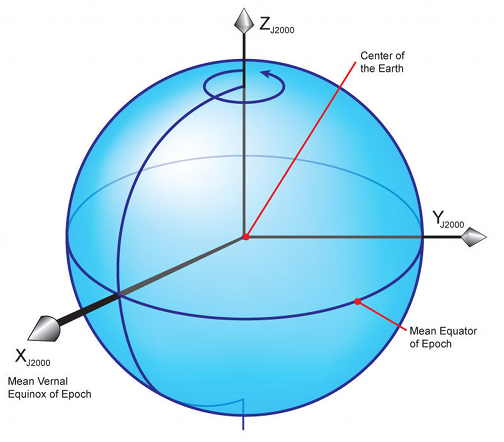
\includegraphics [width=7in]{figs/fig4.png}
\caption{International Celestial Reference Frame}
\label{fig:4}
\end{figure}

\subsection{Example Earth ICRF }
To set up a non-spherical Earth one must invoke a transformation from inertial to body fixed coordinates must be set up. As an example,set up a sim\_object in the S\_define file, for instance see SIM 2 in the \hyperTutorial. Set the coordinate system the S\_define sim object Earth must contain the following parameters, see the \hyperTutorial\ for all variable and parameter definitions:

\begin{verbatim}

// SIM_OBJECT: earth
// This sim object models the space environment.
//=============================================================================
sim_object {

   //
   // Data structures
   //
   environment/planet:  Planet               planet
      (environment/planet/data/earth.d);


   environment/gravity:    SphericalHarmonicsGravityBody   gravity_body
      (environment/gravity/data/earth_GGM02C.d);

   environment/RNP/RNPJ2000:        RNPJ2000             rnp
      (environment/RNP/RNPJ2000/data/rnp_j2000.d);

   environment/RNP/RNPJ2000:        NutationJ2000Init    nut_init
      (environment/RNP/RNPJ2000/data/nutation_j2000.d);

   environment/RNP/RNPJ2000:        PolarMotionJ2000Init pm_init 
      (environment/RNP/RNPJ2000/data/polar_motion/xpyp_daily.d);
      
   //
   // Initialization jobs
   //
   P_ENV (initialization) environment/gravity:
   earth.gravity_body.initialize_body ( );

   P_ENV (initialization) environment/gravity:
   env.gravity.add_grav_source(
      Inout GravityBody & grav_body = earth.gravity_body );

   P_ENV (initialization) environment/planet:
   earth.planet.register_model(
      Inout GravityBody & grav_body   = earth.gravity_body,
      Inout DynManager  & dyn_manager = dynamics.manager );
 
   P_ENV (initialization) environment/RNP/RNPJ2000:
   earth.rnp.initialize(
      Inout DynManager & manager = dynamics.manager );
   
   P_ENV (initialization) environment/RNP/GenericRNP:
   earth.rnp.nutation->initialize(
      In PlanetRotationInit * init = &earth.nut_init );
 
   P_ENV (initialization) environment/RNP/GenericRNP:
   earth.rnp.polar_motion->initialize(
      In PlanetRotationInit * init = &earth.pm_init );

   P_ENV (initialization) environment/RNP/RNPJ2000:
   earth.rnp.update_rnp (
      In TimeTT & time_tt = time.tt,
      In TimeGMST & time_gmst = time.gmst,
      In TimeUT1 & time_ut1 = time.ut1 ); 
   
   P_BODY (initialization) environment/planet:
   earth.planet.initialize( );

   //
   // Environment class jobs
   //
   
   (LOW_RATE_ENV, environment) environment/RNP/RNPJ2000:
   earth.rnp.update_rnp (
      In TimeTT & time_tt = time.tt,
      In TimeGMST & time_gmst = time.gmst,
      In TimeUT1 & time_ut1 = time.ut1 );
   //
   // Derivative class jobs
   //
   P_ENV Idynamics (derivative) environment/RNP/RNPJ2000:
   earth.rnp.update_axial_rotation(
      In TimeGMST & time_gmst = time.gmst );

} earth;
\end{verbatim}
This also contains the propagation of a spacecraft in Earth orbit.
An example of the inertial coordinates are given in input.py file found in the SET\_test/RUN\_4 directory of Tutorial SIM\_4.





\section{Earth Centered Earth Fixed Coordinates ECEF } \label{sec:itrf} 
Within JEOD Earth centered Earth fixed coordinates are referred to as ECEF.
This is a heritage nomenclature. Body fixed coordinates are the frame in which a non-spherical gravitational field is defined. There exist within JEOD the fields GEM-T1 and GGM02C, the first is defined with respect to the ECEF frame, GGM02C uses the International Terrestrial Reference Frame frame. (One notes these frames have only small difference at the Epoch date of J2000.)
ITRF is realized by the locations of a set of points or stations on a tide-free Earth. As measurements and models have improved or changed, these locations have been changed also and the ITRF moves slightly with respect to the physical Earth every few years.
For details see the IERS specification document \cite{IERS2003}. The ITRF system is related to the ICRF system by the Earth orientation model realized by the JEOD \RNP.
Note the body fixed coordinate states can be recorded but cannot be used to initialize a simulation.

\textbf{Coordinate Frame: } Rotating

\begin{itemize}
\item X-axis: The intersection of the prime meridian and the rotation equator of the Earth.
\item Y-axis: Completes a standard, right-handed coordinate frame.
\item Z-axis: The rotation pole of the Earth.
\end{itemize}

\begin{figure}[htp]
\centering
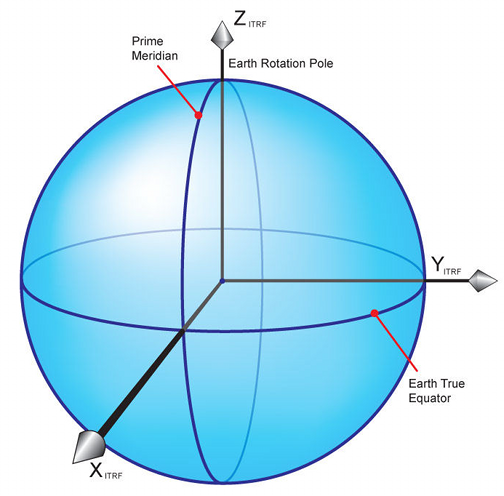
\includegraphics [width=7in]{figs/fig5.png}
\caption{International Terrestrial Reference Frame}
\label{fig:5}
\end{figure}

\subsection{Example ECEF}
See the example in Section 4 \ref{sec:icrf}.
In the Tutorial simulation SIM 2 is an example of recording Earth planet fixed coordinates. 
\begin{verbatim}
earth.planet.pfix.state.rot.T_parent_this[0][0-2]
earth.planet.pfix.state.rot.T_parent_this[1][0-2]
earth.planet.pfix.state.rot.T_parent_this[2][0-2]
\end{verbatim}




\section{Lunar Coordinate System} \label{sec:lunar} 
As noted in section \ref{sec:gen}, all solar system bodies have their inertial coordinate systems center at the body and are co-aligned with the ICRF system. The body fixed system for the Moon is defined in JEOD as principal axis-based lunar coordinate frame to define the directions of the Moon's rotation pole and prime meridian. The transformation from inertial to fixed are provided by the JPL DE421 Ephemerides. 
The numerically integrated physical librations of the Moon are obtained directly from the DE ephemeris file (JPL recommends DE-421, for lunar orientation). The lunar libration paper \cite{LL} defines three (Euler) angles that describe the orientation of the principal axes of the Moon relative to the ICRF reference frame as follows:   
The three Euler angles are
\begin{itemize}
 \item $\phi$ the angle along the ICRF equator, from the ICRF X-axis to the ascending node of the lunar equator; 
 \item $\theta$ the inclination of the lunar equator to the ICRF equator.
 \item $\psi$ the angle along the lunar equator from the node to the lunar prime meridian
 \end{itemize}
The three Euler angles (or libration angles) are illustrated in Figure \ref{fig:6}.

\textbf{Coordinate Frame: } The body centered body fixed frame.

\begin{itemize}
\item X-axis: Points in the direction of the Moon's prime meridian principal axis (minimum moment of inertia).
\item Y-axis: Completes a standard, right-handed coordinate frame.
\item Z-axis: Points in the direction of the Moon's North pole principal axis (maximum moment of inertia).
\end{itemize}

\begin{figure}[htp]
\centering
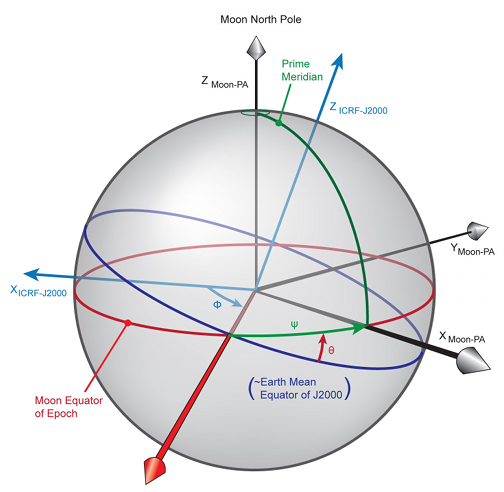
\includegraphics [width=7in]{figs/fig6.png}
\caption{Lunar Inertial and Fixed System}
\label{fig:6}
\end{figure}

\subsection{Example Lunar Coordinate System}
The Moon fixed coordinates are need for computing the non-spherical gravitational accelerations of the Moon.
\begin{verbatim}
An example of setting and recording the Moon's body fixed coordinates can be found in:
\jeod\verif\Integrated_Validation\SIM_Earth_Moon\SET_test\RUN_clem
Set in the input file:
VEH_OBJ.pfix.reference_name     = "Moon";
Recorded in the Log file for the vehicle state:
"#(VEH_OBJ).pfix.state.cart_coords[0-2]";
\end{verbatim}





\section{Mars Coordinate Frames} \label{sec:Mars} 
The generic inertial system for Mars is that defined by the IAU for solar system bodies, namely the ICRF centered on Mars \ref{sec:gen}.
The fixed frame for mars should be the one associated with its fitted gravitational field, see \ref{sec:Marsg}. As of this writing, the Mars gravity model will be MRO110B \cite{2011Icar}. For this document the fixed frame will be that defined by the IAU \ref{sec:gen}.\

\textbf{Coordinate Frame: } Rotating 

\begin{itemize}
\item X-axis: Points in the direction of the prime meridian of Mars.
\item Y-axis: Completes a standard, right-handed coordinate frame.
\item Z-axis: Defined as the pole vector of the Mars Mean Equator.
\end{itemize}

\begin{figure}[htp]
\centering
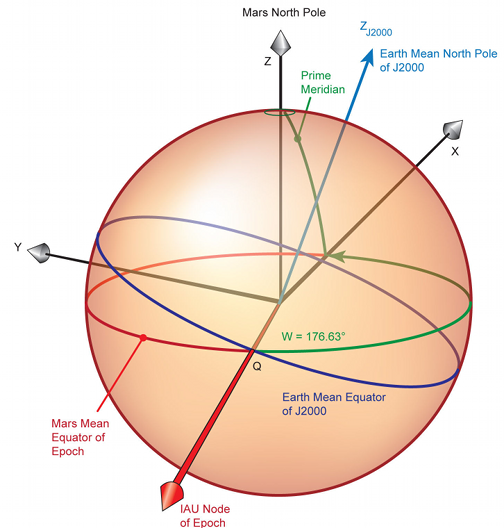
\includegraphics [width=7in]{figs/fig7.png}
\caption{Mars IAU Fixed System}
\label{fig:7}
\end{figure}

\subsection{Example MARS RNP}
See the JEOD \hypermodelref{RNP} for examples.


\section{Mars Gravity Coordinate Frame} \label{sec:Marsg} 
The inertial system for Mars is that defined by the IAU for solar system bodies, namely the ICRF centered on Mars \ref{sec:gen}.
The fixed frame for mars should be the one associated with its fitted gravitational field, see \ref{sec:Marsg}. As of this writing, the Mars gravity model will be MRO110B \cite{2011Icar}.
The document \cite{2006Icar} defines the rotation relation between inertial and fixed coordinates by the angles:
\begin{itemize}
\item The angle N is from the vernal equinox to the node of the Mars mean orbit plane.
\item J is the inclination of Mars mean orbit to the ICRF x-y plane.
\item $\psi$ is the angle from the mean orbit relative to the ICRF x-y plane.
\item I is the inclination of the Mars true equator of date relative to Mars mean orbit.
\item $\phi$ is the spin angle from the node of the Mars true equator of date to prime meridian of Mars, see figure \ref{fig:7a}. 
\end{itemize}

The inertial to Mars fixed transformation is described in JEOD Environment - Mars RNP document.

\textbf{Coordinate Frame: } Rotating 

\begin{itemize}
\item X-axis: Points in the direction of the prime meridian of Mars.
\item Y-axis: Completes a standard, right-handed coordinate frame.
\item Z-axis: Defined as the pole vector of the Mars Mean Equator.
\end{itemize}

\begin{figure}[htp]
\centering
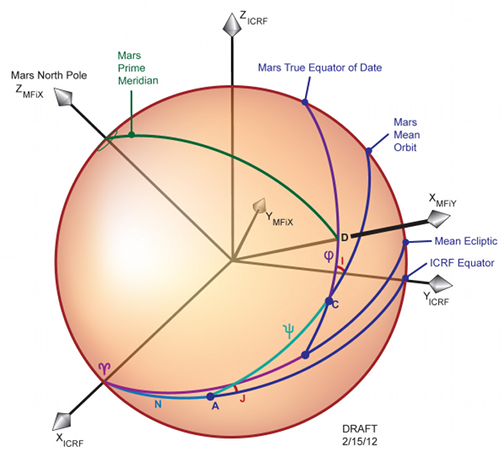
\includegraphics [width=7in]{figs/fig7a.png}
\caption{Mars Gravitational Fixed System}
\label{fig:7a}
\end{figure}

\subsection{Example MARS RNP}
See the JEOD \hypermodelref{RNP} for examples.


\section{Orbital Elements} \label{sec:orb} 
In astrodynamics, the osculating orbit of an object in space (at a given moment of time) is the gravitational Kepler orbit (i.e. ellipse or other conic) that it would have about its central body (corresponding to its actual position and velocity for that given moment of time) if perturbations were not present, see Vallado \cite{Vallado}.

An osculating orbit and the object's position upon it can be fully described by the six standard Keplerian orbital elements (osculating elements), which are easy to calculate as long as one knows the object's position and velocity relative to the central body. The osculating elements would remain constant in the absence of perturbations. However, real astronomical orbits experience perturbations that cause the osculating elements to evolve, sometimes very quickly. In cases where general celestial mechanical analysis of the motion have been carried out (as they have been for the major planets, the Moon, and other planetary satellites), the orbit can be described by a set of mean elements with secular and periodic terms. In the case of minor planets, a system of proper orbital elements has been devised to enable representation of the most important aspects of their orbits.

\textbf{Coordinate Frame:} Quasi-Inertial\\
Base coordinate frame is ICRF as describe in section \ref{sec:gen}.

\begin{itemize}
\item a - is the instantaneous semimajor axis of the orbit.
\item e - is the instantaneous eccentricity of the orbit.
\item i - the inclination of the orbital plane, is the instantaneous angle between the mean inertial north polar axis and the orbital angular momentum vector.
\item $\Omega$ - the right ascension of the ascending node, is the angle measured
eastward from the vernal equinox along the equator to that intersection with
the orbit plane where the vehicle passes from south to north. In the case
where inclination equals zero, the ascending node is defined to be the
X axis of the inertial reference system.
\item $\omega$ -  the argument of perigee, is the angle measured in the orbit plane between the ascending node and perigee, positive in the direction of travel in the orbit. In the case where eccentricity equals zero, perigee is defined to be at the ascending node.
\item $\theta$ the true anomaly, is the geocentric angular displacement of the vehicle measured from perigee in the orbit plane, and positive in the direction of travel in the orbit.
\end{itemize}


\begin{figure}[htp]
\centering
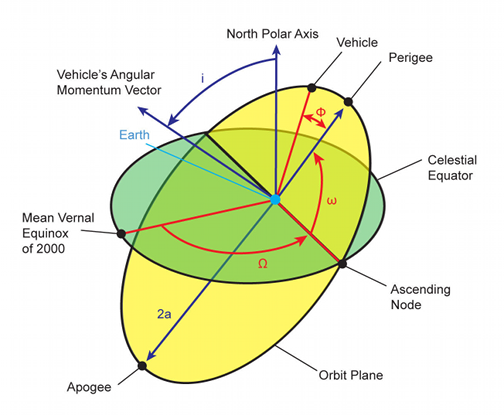
\includegraphics [width=7in]{figs/fig8.png}
\caption{Orbital Elements}
\label{fig:8}
\end{figure}

\subsection{Example Orbital Elements}
See the following JEOD models for an example, \hypermodelref{ORBITALELEMENTS} and \hypermodelref{DERIVEDSTATE}.





\section{Local Vertical Local Horizontal} \label{sec:lvlh} 
Overall crew vehicle guidance, control, navitagion and communications a standard for defining vehile attitudes is usually described based on the standard Euler angle sequence for a space vehicle roll, pitch, and yaw from a 0,0,0 Local Vertical/Local Horizontal (LVLH) coordinate system as in figure \ref{fig:9}. It is possible to pick, roll yaw pitch, pitch yaw roll, pitch roll yaw, yaw roll pitch, or yaw pitch roll as the Euler sequence.

\textbf{Coordinate Frame:} Vehicle-Centered

\begin{itemize}
\item X-axis: Completes a standard, right-handed coordinate frame and is positive in the direction of vehicle motion.
\item Y-axis: Defined as a line that is normal to the orbit plane, positive in the direction opposite to the instantaneous orbit angular momentum vector.
\item Z-axis: Defined as a line that lies along the radius vector from the central body center to the vehicle center-of-mass and is positive toward the central body center.
\end{itemize}

\begin{figure}[htp]
\centering
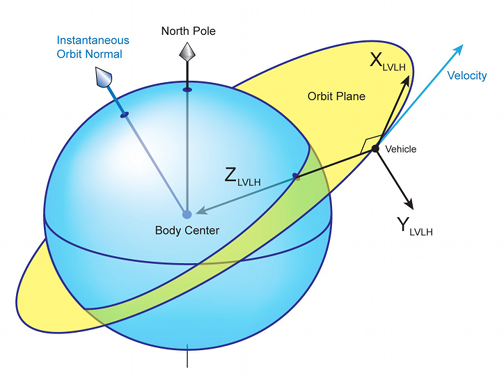
\includegraphics [width=7in]{figs/fig9.png}
\caption{LVLH}
\label{fig:9}
\end{figure}


\subsection{Example LVLH}

See the following JEOD models for an example, \hypermodelref{ORIENTATION} and \hypermodelref{DERIVEDSTATE}.





\section{Body Axis } \label{sec:body} 
A spacecraft body axis associated with a coordinate system fixed in the body itself at its center of mass. This provides a convenient system to refer the vehicle rotational state.
A favored rotation sequence is  an orientation change is subdivided into three consecutive rotations, first around the $x$-axis with angle roll, followed by a rotation around the $y$-axis with angle pitch, and finally another rotation around the actual $z$-axis with angle yaw. 
In order to illustrate this system we pick an example vehicle system as shown in figure \ref{fig:10}

\textbf{Coordinate Frame:} Non-inertial

\begin{itemize}
\item X-axis: positive toward the vehicle cone apex.
\item Y-axis: Parallel to the Vehicle Structural Coordinate System Y-axis, positive toward the crew's right when the crew is seated facing the cone apex.
\item Z-axis: positive in the direction pointing away from the windows and "down" relative to a seated crew member.
\end{itemize}

\begin{figure}[htp]
\centering
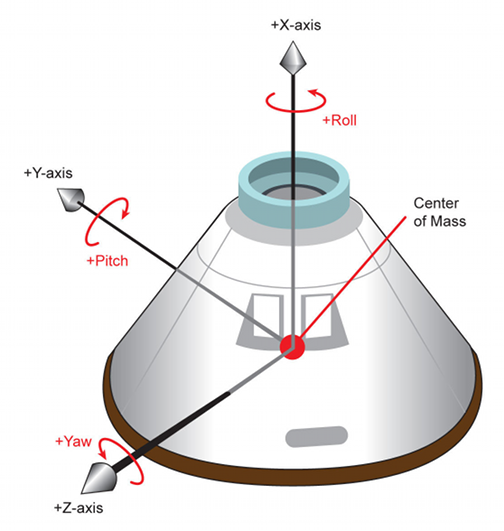
\includegraphics [width=7in]{figs/fig10.png}
\caption{Body Axis}
\label{fig:10}
\end{figure}

\paragraph{Example Body Axis}
See the following JEOD models for an example, \hypermodelref{ORIENTATION} and \hypermodelref{DERIVEDSTATE}.





\section{Structural Frame } \label{sec:struc} 
The structural frame has its history in the frame defined by the
manufacturer of a vehicle for fabrication reference and vehicle body reference operations. It is often defined with the X-axis directed aft, the Y-axis directed toward the right, and the Z-axis directed upward. On some vehicles the centerline serves as the X-axis, with the origin of the coordinate system either at the tip of the vehicle nose, or somewhere out in front of it. Iin the case of the space shuttle, the X-axis was parallel to the longitudinal axis of the payload bay with positive toward the tail, and frame was centered 400 inches below the centerline of the payload bay. A candidate body is picked to demonstrate a structural body axes system.

\textbf{Coordinate Frame:} Non Inertial.

\begin{itemize}
\item X-axis: The X-axis coincides with the centerline of the cone and is positive from the cone apex toward a heat-shield. This orientation , in this example,  is dictated by the use of heritage Shuttle hardware as components.
\item Y-axis:Completes the right-handed system, resulting in the positive direction toward the crew's right when the crew is seated facing the cone apex.
\item Z-axis:The Z-axis lies in the plane containing the origin and a line equidistant between the 2 windows. The positive Z direction corresponds to the "feet to head" direction for the seated crew.
\textbf{The following figure is only an example a user or project is free to choose a convenient structural body axis system.}
\end{itemize}


\begin{figure}[htp]
\centering
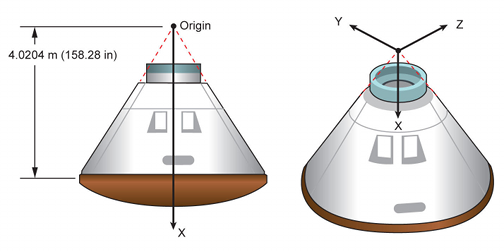
\includegraphics [width=7in]{figs/fig11.png}
\caption{Structural System}
\label{fig:11}
\end{figure}

\subsection{Example Sructural Frame}
For a simple example see:
\begin{verbatim}
jeod\verif\SIM_dyncomp\SET_test\RUN_10A
\end{verbatim}





%%%%%%%%%%%%%%%%%%%%%%%%%%%%%%%%%%%%%%%%%%%%%%%%%%%%%%%%%%%%%%%%%%%%%%%%%
% Bibliography
%%%%%%%%%%%%%%%%%%%%%%%%%%%%%%%%%%%%%%%%%%%%%%%%%%%%%%%%%%%%%%%%%%%%%%%%%

\newpage
\pdfbookmark{Bibliography}{bibliography}
\bibliography{dynenv,COORDFRAME}
\bibliographystyle{plain}

\end{document}

